\section{(Integral) Affine Manifolds}
\frame[c]{\sectionpage}
\begin{frame}[c]{Affine Manifolds}

	\begin{kulblock}{Definition}
		An \textit{affine manifold} is a differentiable manifold such that the transition maps lie in the affine group $\text{Aff}(\R^n)$
	\end{kulblock}
	\begin{remark}
		The group $\text{Aff}(\R^n) := \text{GL}(\R^n) \ltimes \R^n$. An element $g \in \text{Aff}(\R^n)$ acts on $x\in \R^n$ by $g(x) = Ax +b$ where $A \in \text{GL}(\R^n)$ and $b \in \R^n$.
	\end{remark}
\end{frame}

\begin{frame}[c]{(Integral) Affine Manifolds}

	\begin{figure}
		\includegraphics[width=0.6\textwidth]{shearGrid.png}
		\caption{Affine shear transformation}
	\end{figure}
\end{frame}

\begin{frame}[c]{The Affine Connection}

	\begin{kulblock}{Proposition}
		An affine manifold $M$ comes equipped with a flat, torsion free connection
		$\nabla$. In affine coordinates this appears as the standard Euclidean connection.
	\end{kulblock}

	\begin{remark}
		Conversely, a manifold $M$ equipped with a flat, torsion free connection can be endowed with an affine structure.
	\end{remark}
\end{frame}

\begin{frame}[c]{The Development Pair}

	\begin{kulblock}{Lemma (\cite{Ehresmann1936})}
		Let M be an affine manifold and denote by $\tilde{M}$ its universal cover. Then there exists a pair (dev, hol) called the \textit{development pair} where
		$$ \text{dev}: \tilde{M} \to \mathbb{R}^n ,$$
		$$ \text{hol}: \pi_1(M) \to \text{Aff}(\R^n)$$
		The linear part of hol is the holonomy of the affine connection $\nabla$.
	\end{kulblock}

\end{frame}

\begin{frame}[c]{Complete Affine Manifolds}

	\begin{kulblock}{Definition}
		An affine manifold is said to be complete if the development map is a global diffeomorphism. This is equivalent to completeness of the connection $\nabla$.
	\end{kulblock}
	\begin{remark}
		If a discrete group $G$ acts freely and properly on $\R^n$ by affine transformations then $\R^n/G$ will inherit a complete affine structure.
	\end{remark}
\end{frame}

\begin{frame}[c]{Integral Affine Manifolds}

	\begin{kulblock}{Definition}
		An \textit{integral affine manifold} is an affine manifold such that the transition maps lie in the integral affine group $\text{Aff}_{\Z}(\R^n)$ - e.g. the linear part is in $\text{GL}(\Z^n)$
	\end{kulblock}
	\begin{remark}
		An matrix $A \in \text{GL}(\mathbb{Z}^n)$ has $\det A = \pm 1$.
	\end{remark}
\end{frame}

\begin{frame}[c]{Integral Affine Manifolds}

	\begin{kulblock}{Lemma}
		An integral affine structure on a manifold $M^n$ is equivalent to a rank-$n$ lattice in $T^*M$ locally spanned by closed 1-forms
	\end{kulblock}

\end{frame}

\begin{frame}[c]{Examples of Integral Affine Manifolds}

	\begin{itemize}
		\item $\mathbb{R}^n$ with the standard integral affine structure.
		\item The torus $(\mathbb{R}/ \mathbb{Z})^n$ with the integral affine structure
		      induced by translational action of $\mathbb{Z}^n$.
		\item Let $(M, \mathcal{A})$ be an integral affine manifold and suppose that $$f: N
			      \to M$$ is a local diffeomorphism. Then we can pullback the integral affine
		      structure from $M$ to $N$.
	\end{itemize}
\end{frame}

\section{Symplectic geometry and Lagrangian fibrations}
\frame[c]{\sectionpage}
\begin{frame}[c]{Lagrangian Submanifold}
	\begin{definition}[Lagrangian Submanifold]
		Let $(M, \omega)$ be a symplectic manifold and let $N \subset M$ be a submanifold. $N$ is said to be a \emph{Lagrangian submanifold} of $M$
		if $\dim N = \frac{1}{2}\dim M$ and $\omega|_N = 0$.
	\end{definition}
	\begin{example}
		The cotangent bundle $(T^*B, \omega_{can})$ has a canonical symplectic structure. The fibres of $\pi: T^*B \to B$ are Lagrangian submanifolds of $T^*B$.
	\end{example}
\end{frame}

\begin{frame}[c]{Lagrangian Fibration}
	\begin{kulblock}{Definition}
		A Lagrangian fibration $\pi : (M, \omega) \to B$ is a surjective map whose (regular) fibres are Lagrangian submanifolds of $(M, \omega)$.
	\end{kulblock}
	\begin{remark}
		Throughout this talk we will assume that $\pi$ is a surjective submersion and a proper map so that by a theorem of \cite{Ehresmann1951}, $\pi : (M, \omega) \to B$ is a fiber bundle.
	\end{remark}
\end{frame}

\begin{frame}[c]{Examples of Lagrangian Fibrations}
	\begin{itemize}
		\item $(T^*B, \omega_{can}) \to B$ is a Lagrangian fibration.
		\item $(T^*B, \omega_{can} + \pi^*\beta) \to B$ - where $\beta \in \Omega^2(B)$ is closed.
		\item Completely integrable Hamiltonian systems. $(M^{2n}, \omega)$ and $F=f_1, \dots
			      , f_n : M \to \mathbb{R}^n$ with

		      $$\{f_i, f_j\} = 0$$
		      $$df_1 \wedge \dots \wedge df_n \neq 0$$ almost everywhere.
	\end{itemize}
\end{frame}

\begin{frame}[c]{Integral Affine structure on the Base}
	Let $\rho: M \to B$ be a Lagrangian fibration.
	\begin{itemize}
		\item $T_b^*B \circlearrowright M_b$ fibrewise. Given $\alpha \in \Omega^1(B)$ we associate $X_{\alpha} \in \mathfrak{X}(M)$ by
		      $$ \iota_{X_{\alpha}}\omega = -\rho^*\alpha.$$
		\item Denoting the time $1$ flow of $X_{\alpha}$ by $F_{\alpha} : M \to M$ this is a
		      fibrewise transitive, vector bundle action of $T^*B$ on $M$.
	\end{itemize}
\end{frame}

\begin{frame}[c]{Integral Affine structure on the Base}
	Let $\Lambda \subset T^*B$ be the bundle of stabilisers for this action.
	\begin{kulblock}{Lemma}
		$\Lambda$ is a discrete subbundle of $T^*B$ locally spanned by closed one-forms. In fact, the symplectic
		form $\omega_{can}$ descends to the quotient and $\pi :T^*B/\Lambda \to B$ is a Lagrangian fibration.
	\end{kulblock}
	\begin{remark}
		The lattice $\Lambda \subset T^*B$ gives $B$ the structure of an integral affine manifold.
	\end{remark}
\end{frame}

\begin{frame}[c]{Integral Affine structure on the Base}
	\begin{kulblock}{Definition}
		The Lagrangian fibration $\pi :T^*B/\Lambda \to B$ will be called the symplectic reference Lagrangian fibration with period lattice $\Lambda$.
	\end{kulblock}
\end{frame}

\begin{frame}[c]{Integral Affine structure on the Base}
	\begin{kulblock}{Lemma}
		Let $M \to B$ and $M' \to B$ be Lagrangian fibrations. Then if there is a fibrewise symplectomorphism
		covering the identity $\varphi: M \to M'$ then the induced integral affine structure on $B$ is the same for both fibrations.
	\end{kulblock}

	\begin{remark}
		The converse for this does not hold. Adding a non-exact, closed 2-form to $(T^*B, \omega_{can})$ is an example.
	\end{remark}
\end{frame}

\section{Classifying Integral Affine Structures}
\frame[c]{\sectionpage}
\begin{frame}[c]{Classifying Complete Integral Affine Structures}
	\begin{itemize}
		\item Completeness forces injectivity of holonomy representation
		\item Classifying complete structures $\longleftrightarrow$ classifying injective
		      holonomy representations inducing free and proper action on $\R^n$.
	\end{itemize}
\end{frame}

\begin{frame}[c]{Possible Compact Affine Surfaces}
	\begin{kulblock}{Theorem (Milnor)}
		If M is a compact, orientable surface of genus $g\geq 2$, then it does not possess a flat affine connection.
	\end{kulblock}

	\begin{corollary}
		The only possible orientable compact surfaces admitting an (integral) affine structure are sphere $S^2$ and the torus $T^2$
	\end{corollary}
\end{frame}

\begin{frame}[c]{Possible Compact Affine Surfaces}
	\begin{kulblock}{Lemma}
		$S^2$ does not admit an (integral) affine structure
	\end{kulblock}

	\begin{corollary}
		The only compact integral affine surfaces are the torus and Klein bottle.
	\end{corollary}
\end{frame}

\begin{frame}[c]{Nilpotent Holonomy}
	\begin{kulblock}{Theorem (\cite{nilpotent-holonomy})}
		Let $M$ be an orientable, compact affine manifold with nilpotent holonomy group. Then $M$ is complete if and only if it possesses a parallel volume form.
	\end{kulblock}

	\begin{corollary}
		A compact, orientable, integral affine surface with nilpotent holonomy is complete.
	\end{corollary}
\end{frame}

\begin{frame}[c]{Nilpotent Holonomy}
	\begin{itemize}
		\item $\pi_1(T^2) =  \mathbb{Z} \times \mathbb{Z}$
		\item $\pi_1(K^2) = \langle a,b \mid aba = b \rangle$
	\end{itemize}
	\begin{center}
		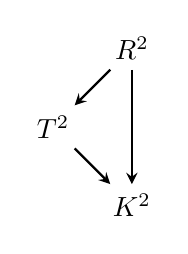
\begin{tikzpicture}[>=stealth, thick]

			% Nodes
			\node (X) at (0,2) {$\mathbb{R}^2$};
			\node (B) at (0,0) {$K^2$};
			\node (Bhat) at (-1,1) {$T^2$};

			% Arrows
			\draw[->] (X) -- (B);
			\draw[->] (X) -- (Bhat);
			\draw[->] (Bhat) -- (B);

		\end{tikzpicture}
	\end{center}
\end{frame}

\begin{frame}[c]{Nilpotent Holonomy}
	\begin{kulblock}{Corollary}
		Any integral affine structure on the 2-torus or the Klein bottle is complete.
	\end{kulblock}
\end{frame}

\begin{frame}[c]{Classification of Integral Affine Structures on $\mathbb{T}^2$ - $\pi_1(T^2) =  \mathbb{Z} \times \mathbb{Z}$}
	\begin{kulblock}{Theorem (\cite{MISHACHEV1996301})}
		The possible generators for the affine holonomy group are
		\begin{enumerate}
			\item $(I, \begin{pmatrix}
					      a \\ c
				      \end{pmatrix})$ and $(I, \begin{pmatrix}
					      b \\ d
				      \end{pmatrix})$ with $\det(\begin{pmatrix}
					      a & b \\ c & d
				      \end{pmatrix}) \neq 0$ with $a,b,c,d \in \R$

			\item $(I, \begin{pmatrix}
					      a \\ 0
				      \end{pmatrix})$ and $(\begin{pmatrix}
					      1 & n \\ 0 & 1
				      \end{pmatrix}, \begin{pmatrix}
					      0 \\ b
				      \end{pmatrix})$ with $n \in \N$ and $a,b >0$
		\end{enumerate}
	\end{kulblock}
\end{frame}

% \begin{frame}[c]
% 	Two integral affine structures of the first type are isomorphic if and only if
% 	\[
% 		X = G X' H
% 	\]
% 	where
% 	\[
% 		X = \begin{pmatrix} a & b \\ c & d \end{pmatrix},
% 		\qquad
% 		X' = \begin{pmatrix} a' & b' \\ c' & d' \end{pmatrix},
% 	\]
% 	and $G, H$ are some matrices from $\mathrm{GL}(2, \mathbb{Z})$.
% \end{frame}

\begin{frame}[c]{Classification of Integral Affine Structures on $\mathbb{K}^2$ - $\pi_1(K^2) = \langle a,b \mid aba = b \rangle$}
	Let $A_1 = \begin{pmatrix}
			1 & n \\ 0 & 1
		\end{pmatrix}$, $A_2 = \begin{pmatrix}
			1 & n \\ 0 & 1
		\end{pmatrix}$ and $B_1 = \begin{pmatrix}
			1 & 0 \\ 0 & -1
		\end{pmatrix}$, $B_2 = \begin{pmatrix}
			0 & 1 \\ 1 & 0
		\end{pmatrix}$
	$B_3 = \begin{pmatrix}
			1 & 1 \\ 0 & -1
		\end{pmatrix}$
	\begin{kulblock}{Theorem (\cite{Sepe2010})}
		The possible generators for the affine holonomy group are
		\begin{enumerate}
			\item $(I, x\textbf{e}_2)$ and $(B_1, y\textbf{e}_1)$ with $x,y > 0$.
			\item $(A_1, x\textbf{e}_2)$ and $(B_1, y\textbf{e}_1 + x\textbf{e}_2)$ with $x,y > 0$.
			\item $(I, x(\textbf{e}_1 - \textbf{e}_2))$ and $(B_2, y\textbf{e}_2)$ with $x,y > 0$.
			\item $(A_2, x\textbf{e}_2)$ and $(B_3, y\textbf{e}_1 + \frac{n-1}{n}x\textbf{e}_2)$ with $2y \neq\frac{n-1}{n}x$ and $x>0$.
		\end{enumerate}
	\end{kulblock}
\end{frame}

\section{Classification of Lagrangian Fibrations}

\frame[c]{\sectionpage}
\begin{frame}[c]{Goal}
	\begin{itemize}
		\item Classify Lagrangian fibrations up to fibrewise symplectomorphism covering the
		      identity.
	\end{itemize}
	\begin{center}
		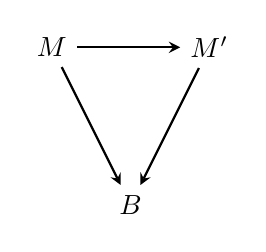
\begin{tikzpicture}[>=stealth, thick]

			% Nodes
			\node (X) at (0,2) {$M$};
			\node (B) at (1,0) {$B$};
			\node (Bhat) at (2,2) {$M'$};

			% Arrows
			\draw[->] (X) -- (B);
			\draw[->] (X) -- (Bhat);
			\draw[->] (Bhat) -- (B);

		\end{tikzpicture}
	\end{center}
\end{frame}

\begin{frame}[c]{How to classify the Lagrangian fibrations over a closed surface}
	\begin{itemize}
		\item Classify the integral affine structures on $B$. (done)
		\item Topological classification - given by \emph{Chern Class}
		\item Symplectic classification - given by \emph{Lagrangian Class}
	\end{itemize}
\end{frame}

\begin{frame}[c]{Luttinger Surgery}
	\begin{itemize}
		\item Luttinger surgery allows us to build new Lagrangian fibrations from
		      $T^*B/\Lambda \to B$.
		\item A type of "symplectic" Dehn surgery.
		\item Using this surgery it is possible to produce all Lagrangian fibrations $M \to
			      B$ by:
		      \begin{itemize}
			      \item Performing Luttinger surgery on $T^*B/\Lambda$.
			      \item Adding a cohomology class to the base.
		      \end{itemize}
	\end{itemize}
\end{frame}

\begin{frame}[c]{The Chern Class}
	This will give the obstruction to $M \to B$ admitting a global section.
	\begin{itemize}
		\item Let $\{U_i\}_{i \in \mathbb{N}}$ be a trivialisation of $M \to B$.
		\item Pick sections $s_i$ over $U_i$ of $M \to B$.
		\item For some $\mu_{ij}: U_i \cap U_j \to T^*B/\Lambda$ we have $s_i = \mu_{ij} +
			      s_j $. This defines a one-cocycle and hence an element $\mu \in H^1(B,
			      \mathcal{T}^*B/\Lambda)$ not depending on the choice of $s_i$.
	\end{itemize}
\end{frame}

\begin{frame}[c]{The Chern Class}
	\begin{itemize}
		\item There is a short exact sequence of sheaves $$0 \to \Lambda \to \mathcal{T}^*B
			      \to \mathcal{T}^*B/\Lambda \to 0$$ which leads to a long exact sequence in
		      sheaf cohomology.
		\item $\mathcal{T}^*B$ is a fine sheaf $\implies$ $H^i(\mathcal{T}^*B)=0$ for $i>0$.
		\item This gives an isomorphism $\delta: H^1(B, \mathcal{T}^*B/\Lambda) \to H^2(B,
			      \Lambda)$
	\end{itemize}
\end{frame}

\begin{frame}[c]{The Chern Class}
	Recall:
	\begin{enumerate}
		\item $s_i = \mu_{ij} + s_j $ defines a one-cocycle and hence an element $\mu \in H^1(B, \mathcal{T}^*B/\Lambda)$
		\item $\delta: H^1(B, \mathcal{T}^*B/\Lambda) \to H^2(B,
			      \Lambda)$ is an isomorphism.
	\end{enumerate}
	\begin{kulblock}{Lemma (\cite{ActionAngle})}
		The image of $\mu$ under the isomorphism $\delta$ defines a class $[\mu_C] \in H^2(B,
			\Lambda)$. This class is the obstruction to our bundle $M \to B$ being topologically equivalent to the
		symplectic reference bundle $T^*B/\Lambda \to B$.
	\end{kulblock}
\end{frame}

\begin{frame}[c]{The Lagrangian Class}
	\begin{itemize}
		\item 	If we require the sections of $\mu_{ij}:=s_i - s_j$ to be Lagrangian we define
		      a cohomology class $\hat{\mu}_L \in H^1(\mathcal{Z}(T^*B/\Lambda))$
		\item There is a short exact sequence of sheaves $$0 \to \Lambda \to
			      \mathcal{Z}(\mathcal{T}^*B) \to \mathcal{Z}(\mathcal{T}^*B/\Lambda) \to 0$$
		      which leads to a long exact sequence in sheaf cohomology.
	\end{itemize}
	$$\dots \to H^1(\Lambda) \to
		H^1(\mathcal{Z}(\mathcal{T}^*B)) \to H^1(\mathcal{Z}(\mathcal{T}^*B/\Lambda)) \xrightarrow{\Delta} H^2(\Lambda) \xrightarrow{\hat{d}} H^2(\mathcal{Z}(\mathcal{T}^*B)) \to  \dots$$
\end{frame}

\begin{frame}[c]{Relating the classes}
	\begin{itemize}
		\item We have that $\mu_L \xmapsto{\Delta} \mu_C \xmapsto{\hat{d}} 0$.
		\item A necessary and sufficient condition for an element $\mu$ in $H^2(\Lambda)$ to
		      be the Chern class of some Lagrangian torus fibration is that $\hat{d}(\mu) =
			      0$
		\item Every class $[\mu] \in H^1(\mathcal{Z}(T^*B/\Lambda))$ can be realized as the
		      Lagrangian class of some Lagrangian torus fibration. (Luttinger surgery).
		\item Fixing $\mu_C$ such that $\hat{d}(\mu) = 0$, the elements $\mu_L$ such that
		      $\Delta(\mu_L) = \mu_C$ are classified by a quotient of $H^2(B, \mathbb{R})$
	\end{itemize}
\end{frame}

\begin{frame}[c]{The Torus Classification (\cite{MISHACHEV1996301})}
	The Lagrangian fibrations $M \to \mathbb{T}^2$ are classified by
	\section*{Integral Affine Structure}
	\begin{itemize}
		\item The integral affine structure on the base.
		      \begin{itemize}
			      \item$\mathcal{A}_{a,b,c,d} = \bigg\langle(I, \begin{pmatrix}
						            a \\ c
					            \end{pmatrix}), (I, \begin{pmatrix}
					            b \\ d
				            \end{pmatrix})\bigg\rangle$.

			      \item $\mathcal{B}_{n,a,b} = \bigg\langle (I, \begin{pmatrix}
						            a \\ 0
					            \end{pmatrix}), (\begin{pmatrix}
					            1 & n \\ 0 & 1
				            \end{pmatrix}, \begin{pmatrix}
					            0 \\ b
				            \end{pmatrix}) \bigg\rangle$
		      \end{itemize}
		\item An element $[s] \in H^2(\Lambda)$.
		      \begin{itemize}
			      \item For $\mathcal{A}_{a,b,c,d}$ we have that $H^2(\Lambda) = \mathbb{Z}\oplus
				            \mathbb{Z}$.
			      \item For $\mathcal{B}_{n,a,b}$ we have that $H^2(\Lambda) =
				            \dfrac{\mathbb{Z}}{n\mathbb{Z}}\oplus \mathbb{Z}$
		      \end{itemize}
		\item An element $[h] \in H^2(\mathbb{T}^2, \mathbb{R})/N$ where $N$ is some normal
		      subgroup.
	\end{itemize}

\end{frame}

\begin{frame}[c]{The Klein Bottle Classification (\cite{Sepe2010})}
	The Lagrangian fibrations $M \to \mathbb{K}^2$ are classified by
	\begin{itemize}
		\item The integral affine structure on the base.
		\item An element $[s] \in H^2(\Lambda)$.
		\item $$H^2(\Lambda) = \begin{cases}
				      \dfrac{\mathbb{Z}}{2\mathbb{Z}} \oplus \mathbb{Z}, \quad \text{for family 1) and family 2) with }n\equiv 0 \text{ mod }2. \\
				      \mathbb{Z}, \quad \text{otherwise.}
			      \end{cases}$$
	\end{itemize}
\end{frame}

\begin{frame}[c]{Classification of Integral Affine Structures on $\mathbb{K}^2$ - $\pi_1(K^2) = \langle a,b \mid aba = b \rangle$}
	Let $A_1 = \begin{pmatrix}
			1 & n \\ 0 & 1
		\end{pmatrix}$, $A_2 = \begin{pmatrix}
			1 & n \\ 0 & 1
		\end{pmatrix}$ and $B_1 = \begin{pmatrix}
			1 & 0 \\ 0 & -1
		\end{pmatrix}$, $B_2 = \begin{pmatrix}
			0 & 1 \\ 1 & 0
		\end{pmatrix}$
	$B_3 = \begin{pmatrix}
			1 & 1 \\ 0 & -1
		\end{pmatrix}$
	\begin{kulblock}{Theorem (\cite{Sepe2010})}
		The possible generators for the affine holonomy group are
		\begin{enumerate}
			\item $(I, x\textbf{e}_2)$ and $(B_1, y\textbf{e}_1)$ with $x,y > 0$.
			\item $(A_1, x\textbf{e}_2)$ and $(B_1, y\textbf{e}_1 + x\textbf{e}_2)$ with $x,y > 0$.
			\item $(I, x(\textbf{e}_1 - \textbf{e}_2))$ and $(B_2, y\textbf{e}_2)$ with $x,y > 0$.
			\item $(A_2, x\textbf{e}_2)$ and $(B_3, y\textbf{e}_1 + \frac{n-1}{n}x\textbf{e}_2)$ with $2y \neq\frac{n-1}{n}x$ and $x>0$.
		\end{enumerate}
	\end{kulblock}
\end{frame}

\begin{frame}[c]{Questions?}
	\begin{center}
		\Large Questions?
	\end{center}

\end{frame}
